\section{Previous Work} \label{tex:previous_work}
In this section a recap of some different approaches to speed up or decrease the number of parameters will be given. In 2013 Denil et al. found NNs to be heavily over-parametrized \cite{Denil2013}. They did this by training only a fraction of the weights and using these to predict the rest of the weights. They reported that in some cases more than 95\% of the weights could be predicted, hence would not need to be learned. Ever since, numerous attempts have been proposed to optimise the evaluation time and number of parameters in NNs. One approach have been to decompose the dense layer of a NN, an other have tried speeding up the evaluation of a convolution, and some have had success in decomposing and speeding up an entire network. All the work described below follow approximately the same structure:

\begin{enumerate}
    \item \textbf{Decompose weights of pre-trained NN} using some specific algorithm to get a smaller representation of the weights or filters
    \item \textbf{Changing the evaluation algorithm} in order for it to correspond to original evaluations and in order to do back-propagation
    \item \textbf{Fine-tuning} which is training the network using the new algorithm and back-propagation 
\end{enumerate}
Some approaches will be discussed in the following. In the end the methods will be compared using a set of different metrics. 

\subsection{Decomposing the dense layer}
In 2015 Nokinov et al. used TT-decomposition to decompose the weights of a dense (fully-connected) layer in an ANN\cite{Novikov2015}. This method exploits the power of the dense layer and allows it to have a big amount of neurons. The dense layer performs a linear transformation on an input vector $\bs{x}$ of dimension $N$:
\begin{equation}
    \bs{y} = W \bs{x} + \bs{b}
    \label{eq:linearTransform}
\end{equation}
Where $W \in \R^{M\times N}$ is the weight matrix and $\bs{b} \in \R^{M}$ is the bias vector. $M$ is the dimension of the output $\bs{y}$. Since the weights of the dense layer are given in a matrix, Nokinov et al. folds this matrix into a 3-dimensional tensor in order to decompose it using the TT algorithm. They define the TT-layer to be the same transformation but with the weights stored in the TT-format. Let $\tensor{X}$ be the input tensor of dimension $d$ (formed from $\bs{x}$), and let the decomposition of the weight matrix have cores $G_k[i_k, j_k]$. In the TT-layer the transformation corresponding to \eqref{eq:linearTransform} is given as:
\begin{equation}
    \tensor{Y}(i_1, i_2, \dots, i_d) = \sum_{j_1, j_2, \dots, j_d} G_1[i_1, j_1] G_2[i_2, j_2]\dots G_d[i_d, j_d] \tensor{X}(j_1, j_2, \dots j_d) + \tensor{B}(i_1, i_2, \dots, i_d)
\end{equation}
Where $\tensor{B}$ is the bias tensor. The properties of the TT-format allows for computation of back-propagation, which is then used for fine-tuning the network. The authors report a best-case compression of a dense layer of up to 200,000 times and of a whole network of up to 7.

\subsection{Speeding up the evaluation of a convolution}
In 2013 Rigamonti et al. \cite{Rigamonti2013} found that filters can be computed as a linear combination of smaller separable filters. A filter is called separable when it can be expressed using multiple parts of lower dimension, as for instance using the CP-decomposition as illustrated by \cite{Sironi2015} in \autoref{fig:separable_filters}. Ever since many approaches have been considered using this principle in different ways. For instance Jaderberg et al. proposed two different schemes for using rank-1 filters to exploit the cross-channel / filter redundancy \cite{Jaderberg2014}. Since these schemes did not built upon any decomposition algorithm per se, the approximation of the separated filters was done by numerically minimizing either the $L_2$ reconstruction error or the reconstruction error of the output of the given layer (indirectly). Two other approaches uses standard decomposition algorithms to ease the evaluation time. One was proposed by Lebedev et al. in 2015 and used CP-decomposition to decompose the convolutional kernel \cite{Lebedev2015}, another was proposed by Wang and Cheng in 2016 and used BTD. They will both be discussed in the following.

\begin{figure}
    \centering
    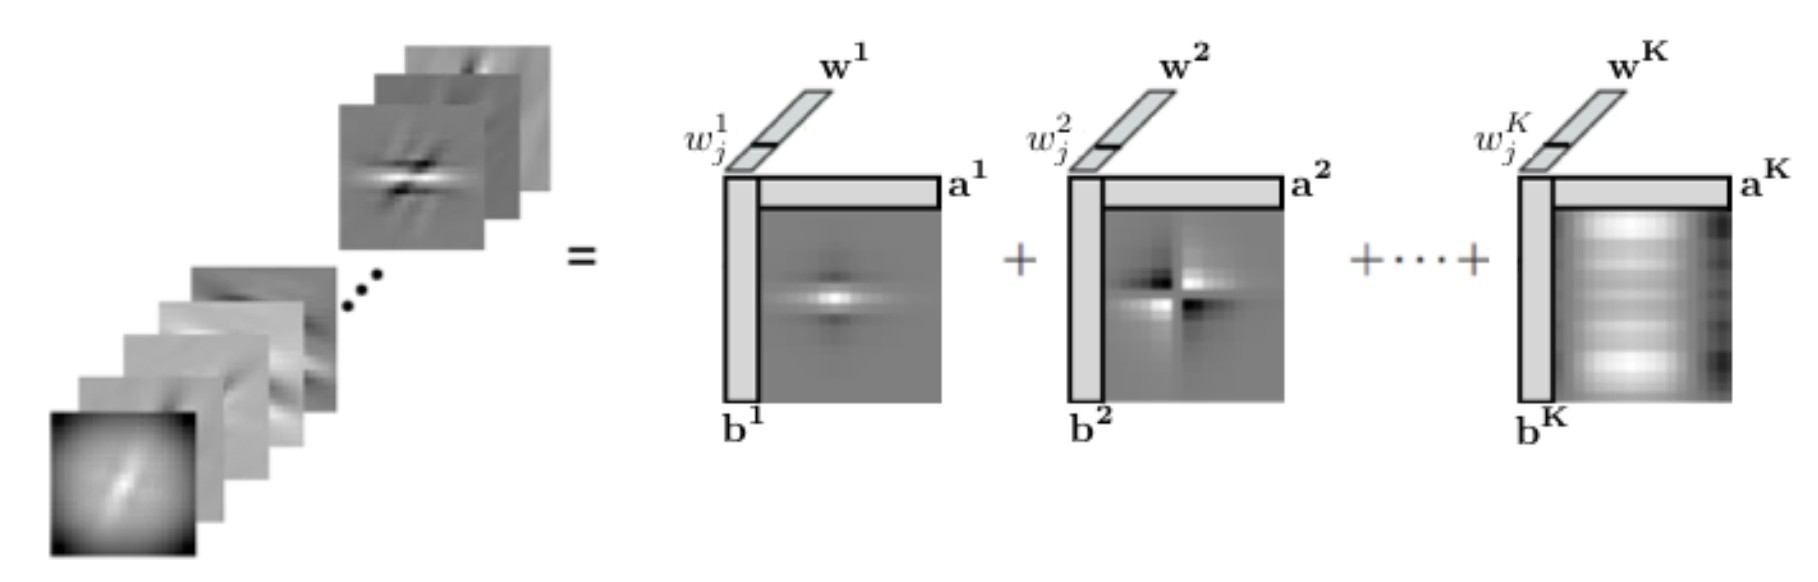
\includegraphics[width=.8\linewidth]{Pics/03_Previous_work/separable_filters.png}
    \caption{Taken from \cite{Sironi2015}. Left: A bank of two-dimensional filters is stacked together to form a 3-dimensional tensor. Right: The tensor is decomposed in the sum of $K$ rank-one tensors. Thus, the original filters are approximated by the weighted sum of the separable filters $s_k = \boldsymbol{a}_k \circ \boldsymbol{b}_k$}
    \label{fig:separable_filters}
\end{figure}

\subsubsection{Convolution using CP-decomposition} \label{tex:convUsingCP}

Lebedev et al. proposed to decompose the 4-dimensional convolutional kernel using CP\Hyphdash decomposition \cite{Lebedev2015}. The idea is to reduce the computation time of the evaluation of a convolutional layer. After having decomposed the kernel into a set of rank-1 tensors, they re-write the convolution into an expression of nested sums using the loadings of the decomposition. The traditional convolution of an input tensor $\tensor{U}$ of size $W \times H \times S$ into an output tensor $\tensor{T}$ of size $(W-d+1)\times (H-d+1)\times t$ looks like this:
\begin{equation}
    \tensor{V}(x, y, t)=\sum_{i=x-\delta}^{x+\delta} \sum_{j=y-\delta}^{y+\delta} \sum_{s=1}^{S} \tensor{K}(i-x+\delta, j-y+\delta, s, t) \ \tensor{U}(i, j, s)
    \label{eq:tradConvolution}
\end{equation}
Where $\tensor{K}$ is the 4-dimensional kernel\footnote{The kernel corresponds to a stack of 3-dimensional filters} of size $d\times d \times s\times t$ and $\delta = \frac{d-1}{2}$ is the half width of the filter in the spatial dimension. Using the decomposition of $\tensor{K}$ with loading matrices $K_w$, $K_h$, $K_s$, and $K_t$, the (approximated) convolution \eqref{eq:tradConvolution} can be written as:
\begin{equation}
    \tensor{V}(x, y, t) = \sum_{r=1}^{R} K_{t}(t, r)\left(\sum_{i=x-\delta}^{x+\delta} K_{w}(i-x+\delta, r)\left(\sum_{j=y-\delta}^{y+\delta} K_{h}(j-y+\delta, r)\left(\sum_{s=1}^{S} K_{s}(s, r) \ \tensor{U}(i, j, s)\right)\right)\right)
\end{equation}
With $R$ being the rank of the decomposition. Now each of the parenthesis can be expressed as intermediate tensors, which means that the whole convolution can be broken into a sequence of four simple convolutions. \autoref{fig:decompConvDifference} shows the difference between a traditional convolution and the sequence of convolutions using the decomposition. The expression of the convolution using the decomposed kernel allows as a sequence of simpler convolutions allows for the use of standard back-propagation. Furthermore it enables easy fine-tuning of the entire network. The authors report that even though the reconstruction error decreases with the increasing rank, a high accuracy is not needed in order to get good prediction results. They also state that their method works well for smaller architectures, while it has a harder time on more complex ones.

\begin{figure}
    \centering
    \begin{subfigure}{\linewidth}
        \centering
        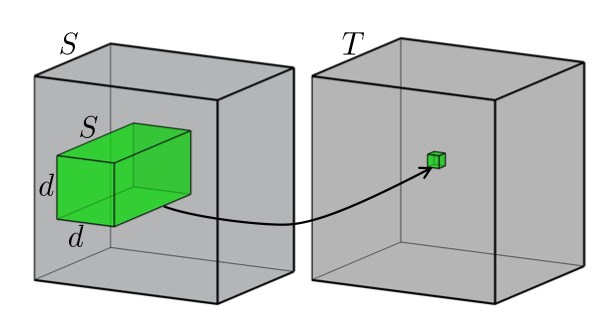
\includegraphics[width=0.4\linewidth]{Pics/03_Previous_work/fullConv.png}
        \caption{Original convolution}
    \end{subfigure}
    \begin{subfigure}{\linewidth}
        \centering
        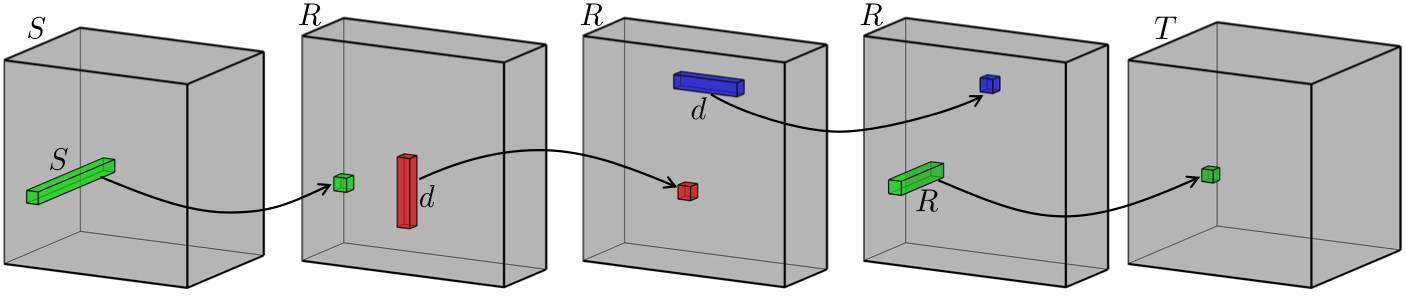
\includegraphics[width=\linewidth]{Pics/03_Previous_work/decompConv.png}
        \caption{Convolution using CP-decomposed kernel}
    \end{subfigure}
    \caption{Taken from \cite{Lebedev2015}. The difference between the original convolution and the sequence of convolutions using the loadings vectors of the CP-decomposition. The grey boxes corresponds to the 3-dimensional tensors within the CNN, with the frontal sides corresponding to the spatial dimension. For instance the first box in each line corresponds to the input image where $S$ is the number of input channels. The arrows show linear mappings, or how to calculate a single value using a filter (top) or a decomposed filter (bottom).}
    \label{fig:decompConvDifference}
\end{figure}

\subsubsection{Convolution using Block Term Decomposition}
Wang and Cheng proposed speeding up the evaluation of a convolution using BTD, which benefits from both sparsity and low-rank. For simplicity they combine the two spatial dimensions into one which means that the convolutional kernel becomes 3-dimensional ($S\times T \times WH$). Since they will not exploit the spatial dimension due to low rank, their decomposition becomes a tucker-2 decomposition of the kernel $\tensor{K}$:

\begin{equation}
    \tensor{K} \approx \sum_{r=1}^{R} \tensor{G}_r \times_1 \bs{A}_r \times_2 \bs{B}_r
\end{equation}

Where $R$ is the rank of the BTD, $\bs{A}_r \in \R^{S\times s}$ and $\bs{B}_r \in \R^{T\times t}$ are the factor matrices along input and output channel dimensions respectively. $\tensor{G}_r \in \R^{s\times t \times P}$ is the core of the $r$'th subtensor. Now the authors concatenate all the $R$ matrices into big matrices $\bs{A}$ and $\bs{B}$. And the core tensors into a big group-sparse core matrix $\tensor{G}$. The result is visualized in \autoref{fig:concatBTD}. The convolution can be done faster using this decomposition and the sequence of convolutions shown in \autoref{fig:BTD_conv_decomp}. The authors also propose a new algorithm for doing the decomposition itself. They call the algorithm Principle Component Iteration (PCI) which is a generalisation of higher order orthogonal iteration (HOOI)

\begin{figure}
    \centering
    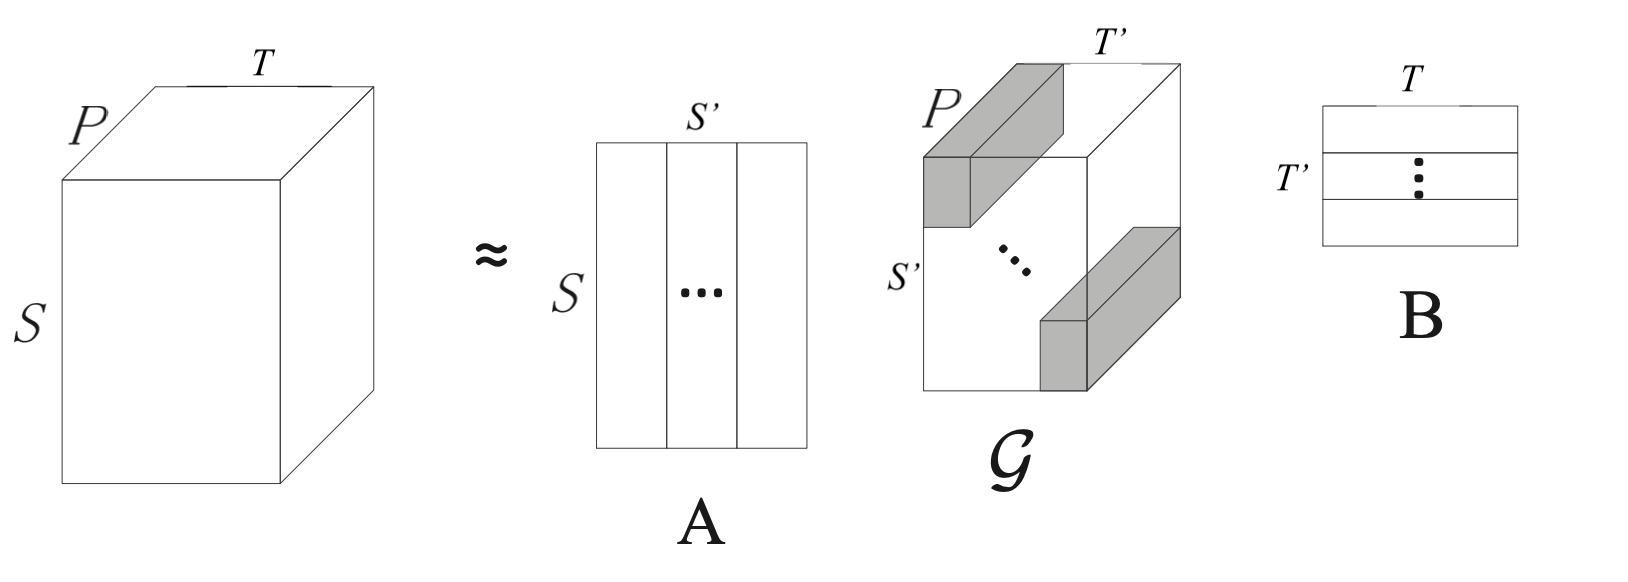
\includegraphics[width=0.8\linewidth]{Pics/03_Previous_work/concatBTD.png}
    \caption{Taken from \cite{Wang2016}. Illustrates how the $R$ factor matrices and core tensors can be concatenated.} 
    \label{fig:concatBTD}
\end{figure}

\begin{figure}
    \centering
    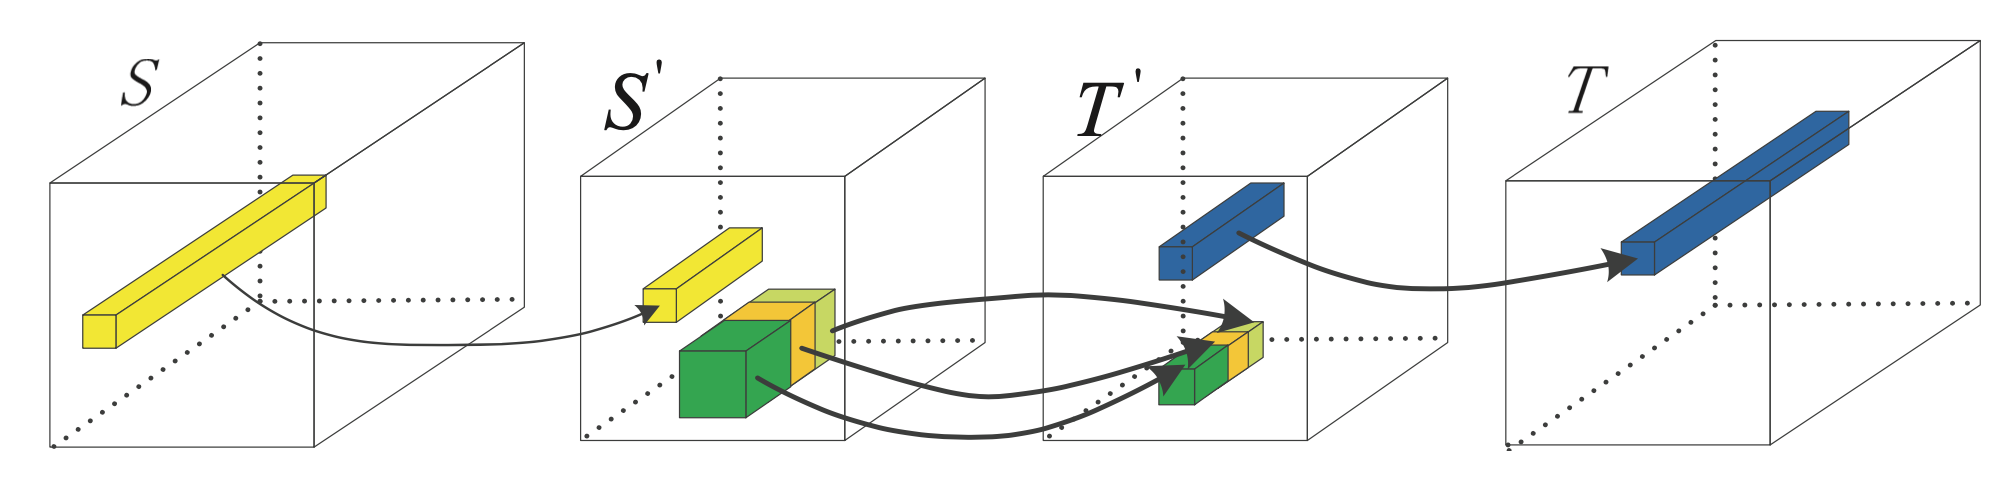
\includegraphics[width=.8\linewidth]{Pics/03_Previous_work/BTD_conv_decomp.png}
    \caption{Taken from \cite{Wang2016}. Illustrates how the convolution is done using the BTD. Each of the boxes correspond to an intermediate tensor with the frontal sides corresponding to spatial dimensions. The arrows show a linear mapping using the factors of the filter.}
    \label{fig:BTD_conv_decomp}
\end{figure}

\subsection{Speeding up the entire network}
All the methods discussed above only describe how to decompose a single layer in the NN; the dense layer or the convolutional layer respectively. In 2016 one method was proposed that would be able to decompose an entire network at once.

Kim et al. proposed using Tucker-decomposition to decompose, not only the convolutional layers, but also the dense layers \cite{Kim2016}. They would use Tucker-2 decomposition from the second convolution to the first dense layer, and Tucker-1 decomposition\footnote{Equivalent to the SVD} for the remaining. They did not decompose the spatial dimensions, since these already are quite small. They also proposed using the global analytical solutions for variational Bayesian matrix factorization (VBMF) developed by Nakajima et al. in 2013 \cite{Nakajima2013} to find the optimal ranks for the decompositions. In a similar derivation to the one in \autoref{tex:convUsingCP}, Kim et al. found that the Tucker-2 decomposed convolutional layer can be described as a sequences of simpler convolutions. This sequence is shown in \autoref{fig:tuckerDecompConv}. They use this sequence to do back-propagation on the entire network at once. The authors report promising results, but states that the optimality of the rank selection needs to be investigated further. They also claim that the $1\times 1$ convolution has great potential and will grow in popularity.\footnote{The yellow and blue convolutions seen in \autoref{fig:tuckerDecompConv}. It is already extensively used in for instance GoogLeNet \cite{Szegedy2015}}

\begin{figure}
    \centering
    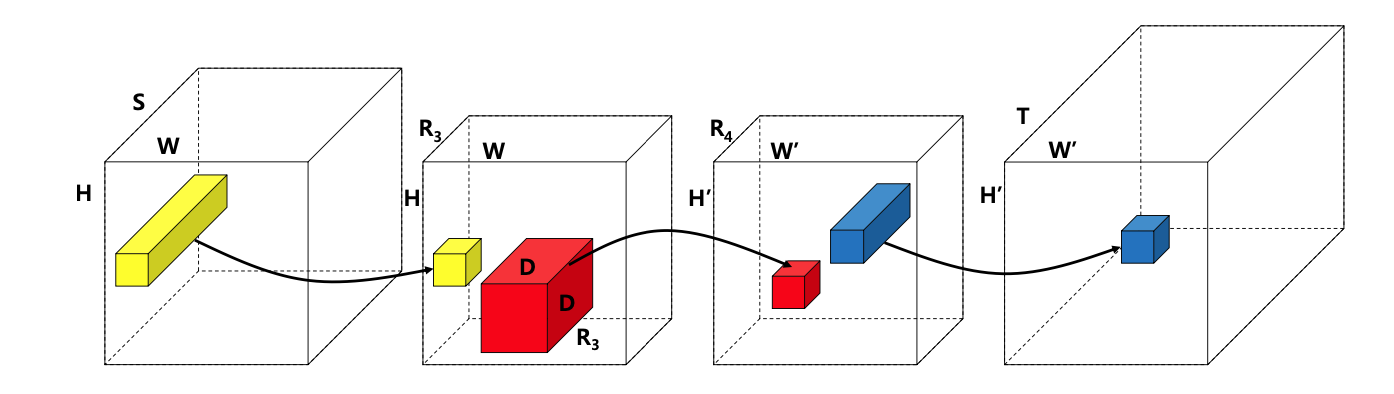
\includegraphics[width=\linewidth]{Pics/03_Previous_work/tuckerDecomp.png}
    \caption{Taken from \cite{Kim2016}. The boxes correspond to the 3-dimensional tensors in the network with the frontal sides being the spatial dimensions. Each of the arrows show a linear mappings. The two middle tensors are the intermediate tensors with $R_3$ and $R_4$ being the ranks of the decomposition.}
    \label{fig:tuckerDecompConv}
\end{figure}

\subsection{Overall comparison of methods}
It seems that the biggest compression happens in the dense layers, since these are very heavy in number of parameters, on the other hand the convolution takes longer since there are more evaluations per parameter. In trying to speed up the CNN, the method using BTD proposed in \cite{Wang2016} seems to get the best results. On the VGG-16 network architecture\cite{Simonyan2015} they achieve an acceleration of $6.6 \times$, while the methods of Jaderberg et al. \cite{Jaderberg2014} and Kim et al. \cite{Kim2016} achieve $3.8 \times$ and $3.3\times$ respectively. The authors of the BTD method also discuss and test decomposing the first dense layer since this can be treated as a convolution with large filters. The method using CP-decomposition \cite{Lebedev2015} worked well, but did not seem to be scaleable.

% Outline:
% Speeding up the dense layer
% Speeding up the convolutional layer
% Speeding up the entire network